\documentclass[border=10pt]{standalone}
\usepackage{tikz}
\usetikzlibrary{arrows.meta,positioning,calc,fit,backgrounds,decorations.pathreplacing}
\usepackage{times}

\begin{document}
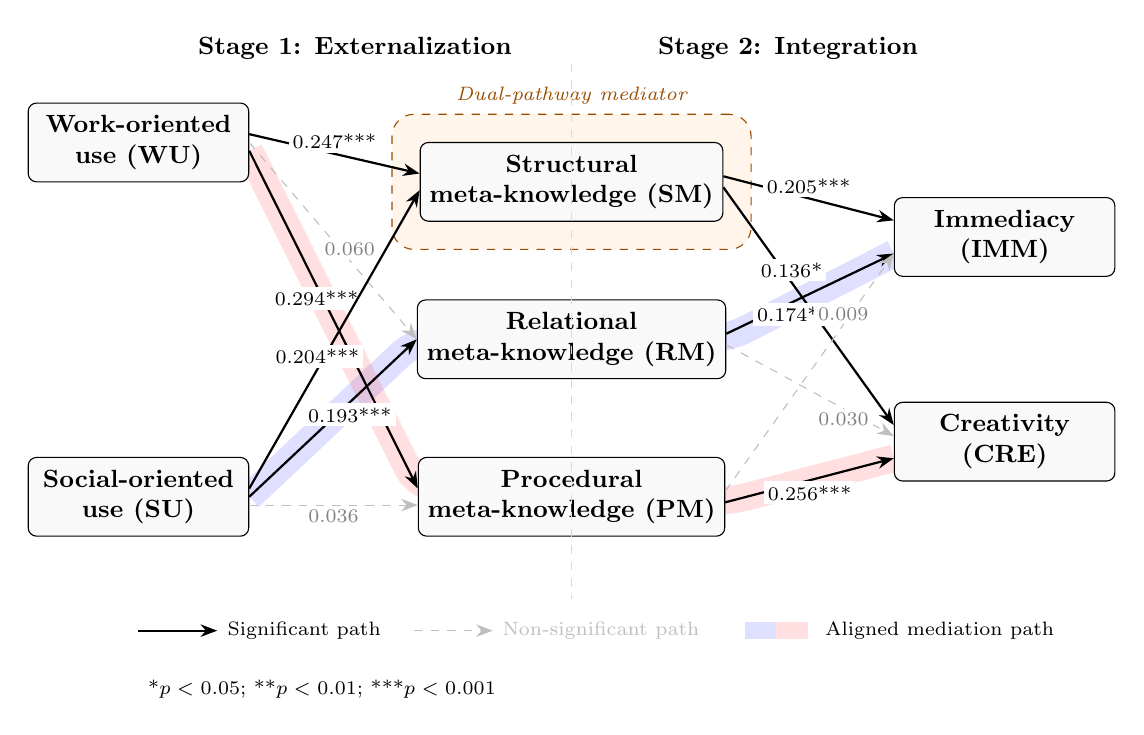
\begin{tikzpicture}[
  % Node styles
  iv/.style={draw, rounded corners=3pt, minimum width=2.8cm, minimum height=1cm,
             font=\small\bfseries, fill=gray!5, align=center},
  mk/.style={draw, rounded corners=3pt, minimum width=2.8cm, minimum height=1cm,
             font=\small\bfseries, fill=gray!5, align=center},
  dv/.style={draw, rounded corners=3pt, minimum width=2.8cm, minimum height=1cm,
             font=\small\bfseries, fill=gray!5, align=center},
  % Arrow styles
  sig/.style={-{Stealth[length=6pt]}, thick, black},
  nonsig/.style={-{Stealth[length=6pt]}, thin, gray!50, dashed},
  % Label style
  lbl/.style={font=\scriptsize, fill=white, inner sep=1.5pt},
]

% === Column 1: IVs ===
\node[iv] (WU) at (0, 0) {Work-oriented\\use (WU)};
\node[iv] (SU) at (0, -4.5) {Social-oriented\\use (SU)};

% === Column 2: Mediators ===
\node[mk] (SM) at (5.5, -0.5) {Structural\\meta-knowledge (SM)};
\node[mk] (RM) at (5.5, -2.5) {Relational\\meta-knowledge (RM)};
\node[mk] (PM) at (5.5, -4.5) {Procedural\\meta-knowledge (PM)};

% === Column 3: DVs ===
\node[dv] (IMM) at (11, -1.2) {Immediacy\\(IMM)};
\node[dv] (CRE) at (11, -3.8) {Creativity\\(CRE)};

% === Stage 1 arrows: IV -> MK (6 arrows) ===
% WU paths
\draw[sig]    ([yshift=3pt]WU.east)  -- node[lbl, above]                {0.247***} ([yshift=3pt]SM.west);
\draw[nonsig] (WU.east)              -- node[lbl, above, pos=0.6, text=gray] {0.060} (RM.west);
\draw[sig]    ([yshift=-3pt]WU.east) -- node[lbl, below, pos=0.4]       {0.294***} ([yshift=3pt]PM.west);

% SU paths
\draw[sig]    ([yshift=3pt]SU.east)  -- node[lbl, above, pos=0.4]       {0.204***} ([yshift=-3pt]SM.west);
\draw[sig]    (SU.east)              -- node[lbl, below, pos=0.6]        {0.193***} (RM.west);
\draw[nonsig] ([yshift=-3pt]SU.east) -- node[lbl, below, text=gray]     {0.036} ([yshift=-3pt]PM.west);

% === Stage 2 arrows: MK -> DV (6 arrows) ===
% SM -> IMM, SM -> CRE (dual-pathway)
\draw[sig] ([yshift=2pt]SM.east)  -- node[lbl, above]           {0.205***} ([yshift=6pt]IMM.west);
\draw[sig] ([yshift=-2pt]SM.east) -- node[lbl, above, pos=0.4]  {0.136*} ([yshift=6pt]CRE.west);

% RM -> IMM (sig), RM -> CRE (n.s.)
\draw[sig]    ([yshift=2pt]RM.east)  -- node[lbl, below, pos=0.4]            {0.174**} ([yshift=-6pt]IMM.west);
\draw[nonsig] ([yshift=-2pt]RM.east) -- node[lbl, below, pos=0.7, text=gray] {0.030} ([yshift=2pt]CRE.west);

% PM -> IMM (n.s.), PM -> CRE (sig)
\draw[nonsig] ([yshift=2pt]PM.east)  -- node[lbl, above, pos=0.7, text=gray] {0.009} ([yshift=-6pt]IMM.west);
\draw[sig]    ([yshift=-2pt]PM.east) -- node[lbl, below]                     {0.256***} ([yshift=-6pt]CRE.west);

% === Background: SM universal zone (only around SM node) ===
\begin{scope}[on background layer]
  \node[fit=(SM), fill=orange!8, draw=orange!60!black, dashed,
        rounded corners=8pt, inner sep=10pt,
        label={[font=\scriptsize\itshape, text=orange!60!black, align=center]above:
          Dual-pathway mediator}] {};
\end{scope}

% === Alignment highlight bands ===
% Aligned path 1: SU -> RM -> IMM (blue)
\begin{scope}[on background layer]
  \draw[blue!70, line width=10pt, rounded corners=8pt, opacity=0.18]
    (SU.east) -- (RM.west) -- (RM.east) -- ([yshift=-6pt]IMM.west);
\end{scope}

% Aligned path 2: WU -> PM -> CRE (red)
\begin{scope}[on background layer]
  \draw[red!70, line width=10pt, rounded corners=8pt, opacity=0.18]
    ([yshift=-3pt]WU.east) -- ([yshift=3pt]PM.west) -- ([yshift=-2pt]PM.east) -- ([yshift=-6pt]CRE.west);
\end{scope}

% === Stage labels (centered over respective arrow zones) ===
\node[font=\small\bfseries] at (2.75, 1.2) {Stage 1: Externalization};
\node[font=\small\bfseries] at (8.25, 1.2) {Stage 2: Integration};

% Subtle vertical separator
\draw[gray!30, thin, dashed] (5.5, 1.0) -- (5.5, -5.8);

% === Legend (horizontal, centered) ===
\draw[sig]    (0.0, -6.2) -- ++(1.0,0) node[right, font=\scriptsize] {Significant path};
\draw[nonsig] (3.5, -6.2) -- ++(1.0,0) node[right, font=\scriptsize] {Non-significant path};
\draw[blue!70, line width=6pt, opacity=0.18] (7.7, -6.2) -- ++(0.4,0);
\draw[red!70, line width=6pt, opacity=0.18]  (8.1, -6.2) -- ++(0.4,0)
  node[right, font=\scriptsize, text=black, opacity=1] {Aligned mediation path};
\node[font=\scriptsize, anchor=north west] at (0.0, -6.7) {*$p < 0.05$; **$p < 0.01$; ***$p < 0.001$};

\end{tikzpicture}
\end{document}
